\section{Example 2: Data Assimilation}

In the last section we used random variables in simple examples involving
discrete random variables, in particular six sided dice. These problems were
solved internally by iteration as done by Erwig et al \cite{Erwig2006}. In this
section, we consider continuous random variables. Instead of iterating through
the continuum of possible values, we generate and solve integral expressions.
 While the backend mechanics have been completely changed, the
method of setting up the statistical problem remains unchanged. This is an
advantage of integrating uncertainty in the language, a theme upon which we
will elaborate in the following sections.

Consider the problem of data assimilation. On a hot summer day, one might guess
the temperature outside to be about $30C$. The uncertainty of this guess can be
encapsulated by an error of $\pm3C$. In SymPy one can model model this estimate
with a normal random variable:

\begin{lstlisting}
>>> T = Normal(30, 3)
\end{lstlisting}

As in the last section, we may ask statistical questions such as ``What is the
probability that the temperature is greater than 33C?'' (i.e. $P(T>33)$). Such
questions produce integral expressions which are then solved using the SymPy
integration engine to produce numeric results.
\begin{eqnarray*}
P(T>33) & = & \int_{33}^{\infty} \frac{\sqrt{2} e^{- \frac{1}{18} \left(x -30\right)^{2}}}{6 \sqrt{\pi}}\, dx \\
& = & - \frac{1}{2} \operatorname{erf}{\left (\frac{1}{2} \sqrt{2} \right )} + \frac{1}{2} \\
& = & 0.15866
\end{eqnarray*}

Unsatisfied with this single estimate of the temperature, we want to update the
our understanding with measurements from a thermometer. However, the thermometer is difficult to read because the lines are spaced closely
together.  This means that our observations will include some noise, which we
include in our model below:

\begin{lstlisting}
>>> noise = Normal(0, 1.5)
>>> observation = T + noise
\end{lstlisting}

The thermometer measures a value of $26C$. We now have two pieces of
information to model the temperature: the measured data ($26\pm1.5C$) and our \textit{prior}
understanding ($30\pm3C$). We plot them both in Fig. \ref{fig:DA_data}.

\begin{figure}[ht]
\vspace{-0pt}
\centering
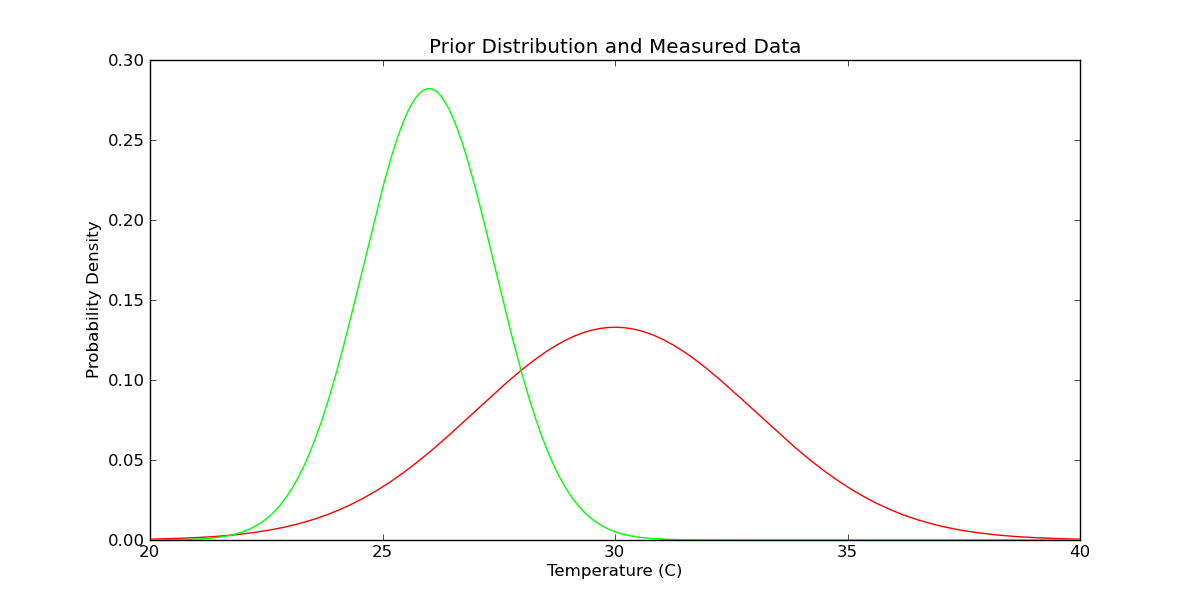
\includegraphics[width=.7\textwidth]{images/data.png}
\vspace{-0pt}
\caption{The probability density functions of our two pieces of data. Note that the observation is less uncertain and thus more centered about the mean.}
\label{fig:DA_data}
\vspace{00pt}
\end{figure}

After this measurement is made how should the final estimate of the temperature change? We have the original estimate, $30 \pm 3C$, and the new measurement $26 \pm 1.5C$. One could select the thermometer's reading because it is more precise but this entirely neglects the original information which still holds some value. It would be best to cleanly assimilate the new bit of data $(26C \pm 1.5C)$ into the prior understanding $(30C \pm 3C)$

This is the problem of Data Assimilation. We want to assimilate a new
measurement (data) into our previous understanding (prior) to form a new and
better-informed understanding (posterior). That is we want to compute $T' = T$
given an observation of $26C$. We compute this in SymPy as follows:

\begin{lstlisting}
>>> T_posterior = Given(T, Eq(observation, 26))
\end{lstlisting}

The new distribution is plotted in Fig. \ref{fig:DA_posterior}. The exact
functional form is proportional to $e^{-\frac{2}{9} \left(-x + 26\right)^{2}}
e^{-\frac{1}{18} \left(x-30\right)^{2}}$

\begin{figure}[ht]
\vspace{-0pt}
\centering
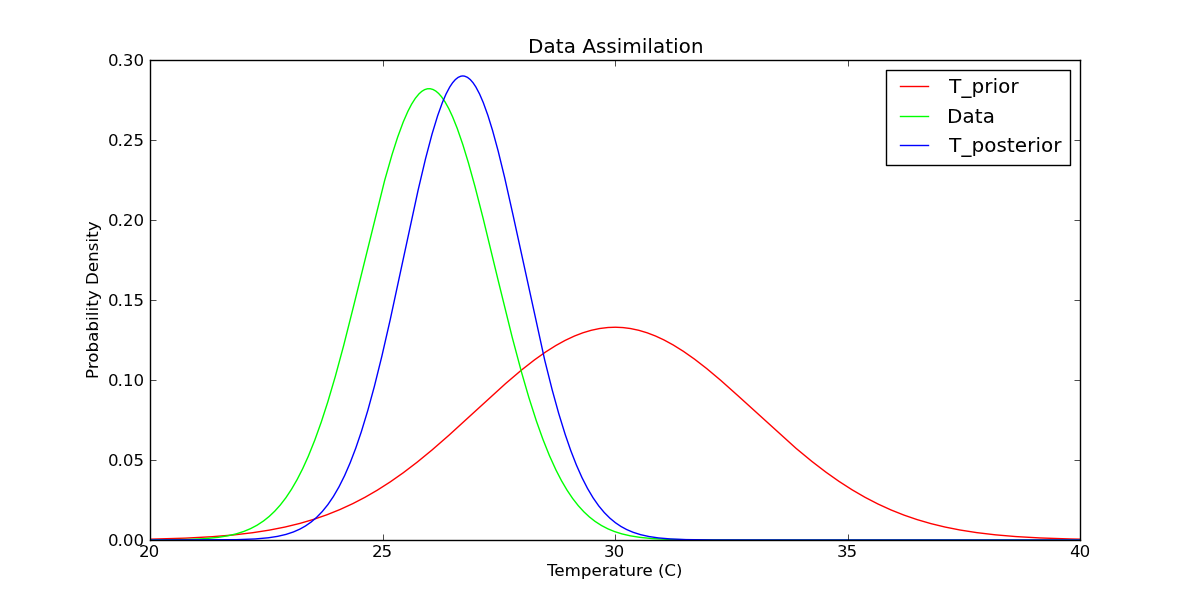
\includegraphics[width=.7\textwidth]{images/posterior.png}
\vspace{-0pt}
\caption{The density of the posterior represents our understanding after the observation has been assimilated into our prior understanding. Note that it is more centered/certain than either of the two. }
\label{fig:DA_posterior}
\vspace{00pt}
\end{figure}

This is a classic result in data assimilation. It is important to note that
the rules for this particular example of data assimilation are not explicitly written into SymPy. Rather the fundamental rules which are coded in SymPy cause this and many other classical results to develop naturally. 
